\chapter{Development of an open-source dashboard for team communication experiments}
\label{ch:dashboard}

The goal of this task was to create an open-source dashboard for controlling
and visualizing team communication experiments in real-time - i.e., to put a
more user-friendly interface on our existing backend infrastructure so that
other researchers at UArizona can utilize it more easily.

\section{Milestones}

We were able to partially complete Milestone 1 (real-time visualization of
automated transcriptions, dialog act classifications, and sentiment labels).
Specifically, we are able to now visualize automated transcriptions in
real-time (see \autoref{fig:asr_viz}). 
We did not implement visualization of dialog act classifications and sentiment
labels, but given our now-increased expertise in working with our visualization
libraries, we expect that it will not be too hard to implement those additions. 


\begin{figure}
    \centering
    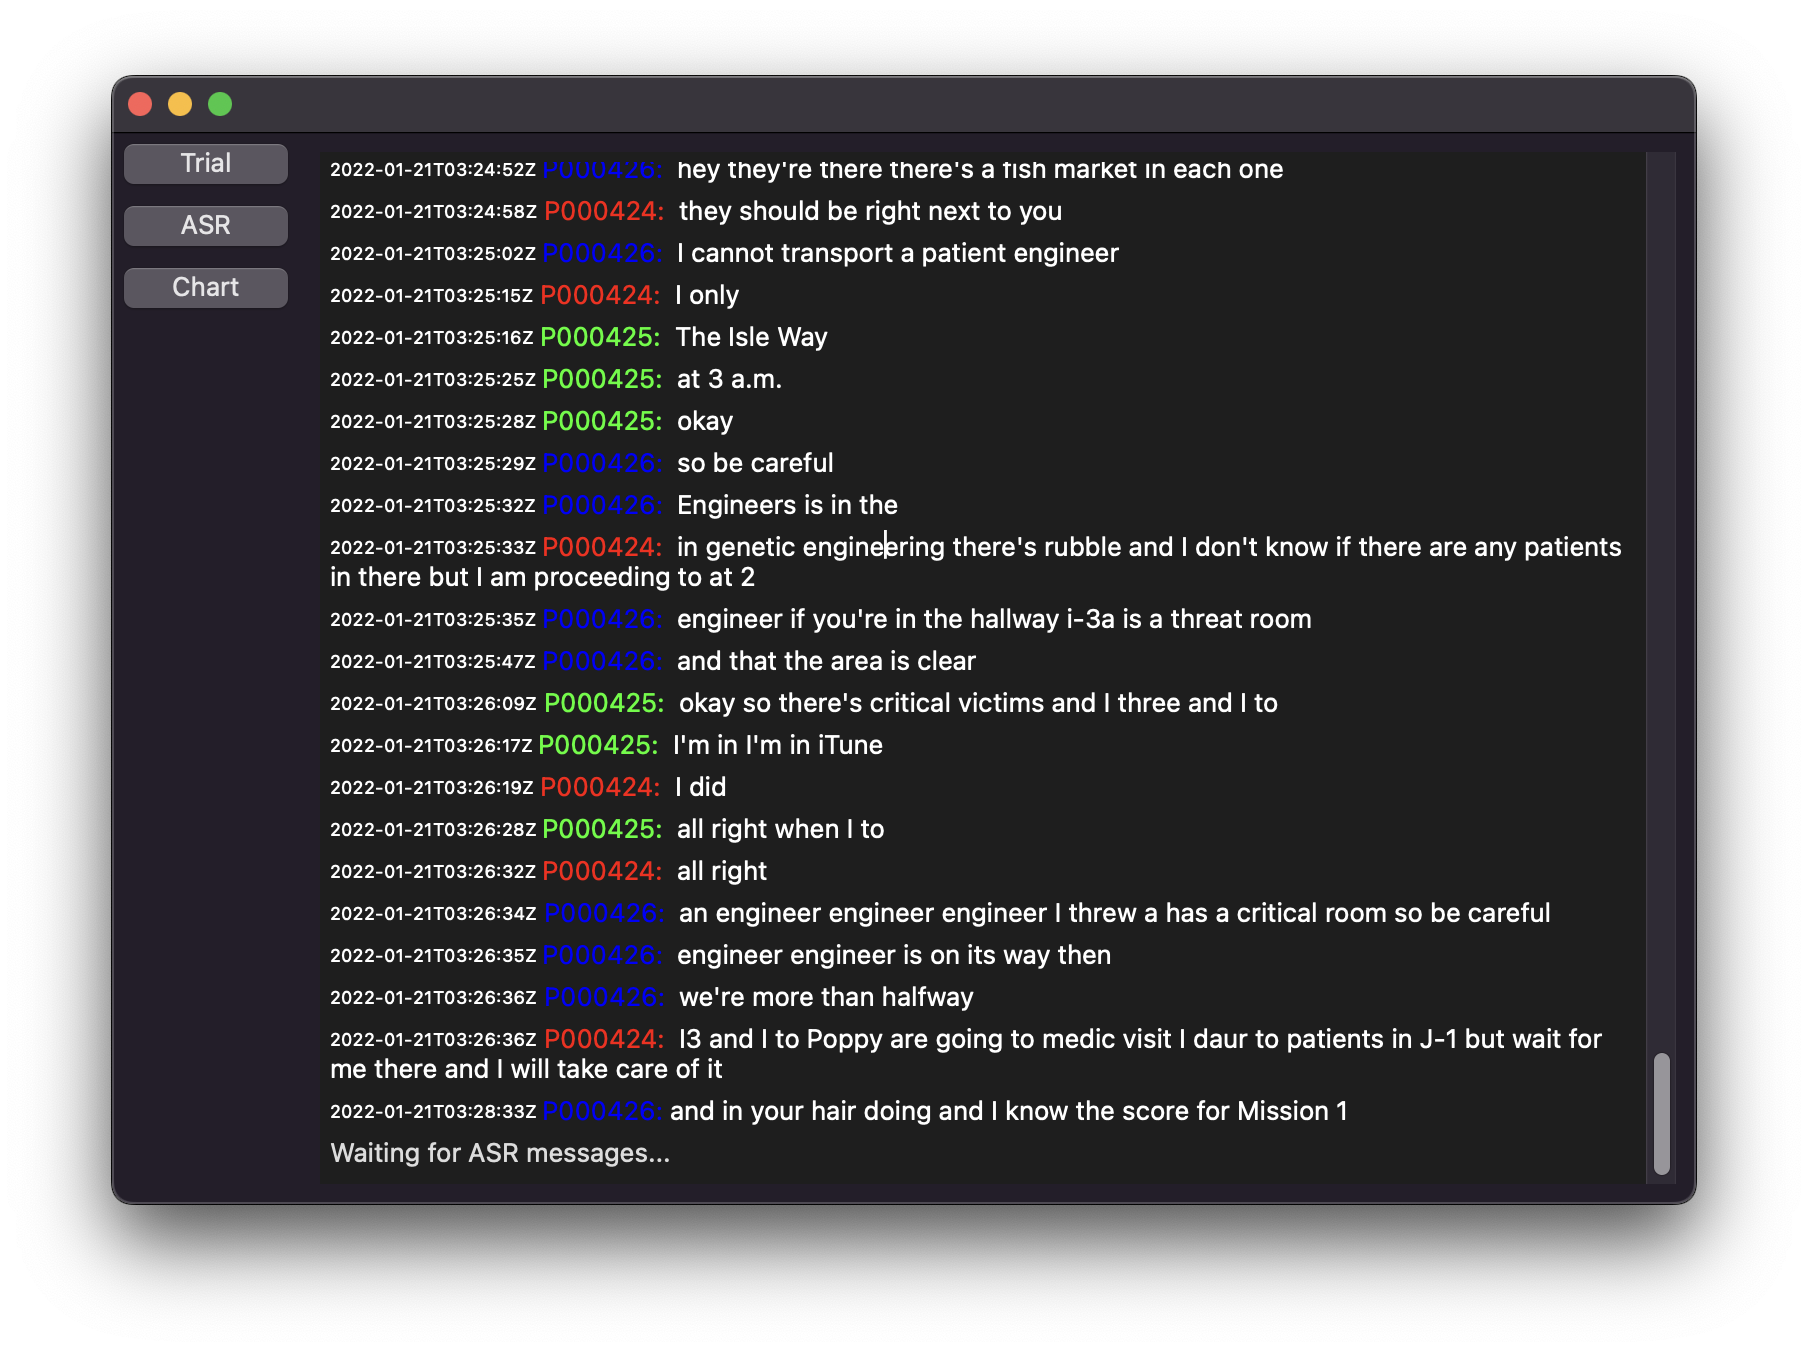
\includegraphics[width=\textwidth]{figures/asr_viz}
    \caption{ASR visualization during ongoing trial.}
    \label{fig:asr_viz}
\end{figure}


We were not able to complete Milestone 2, since this milestone depended on the
development of the WASD sensors (\autoref{sec:wasd}), which we were not able to
complete on time.

In addition to these milestones, we implemented a generic interface for
real-time visualization of scalar values in dynamically updating charts.

In section \autoref{sec:dashboard-quickstart}, we provide a `quickstart' guide
for developers and users of the dashboard.

\section{Current state and future plans}

While the dashboard is currently functional, it is definitely still a
prototype. Additional is needed to (i) make it more robust, and (ii) package it
for easier usage by non-programmers. In the process of developing the
dashboard, we built in-house expertise with wxWidgets, a C++ library for
building native GUIs. We chose to go the native GUI route via C++ as we wished
to minimize resource consumption and improve maintainability by using a
statically typed, compiled language.

We plan to deploy and battle-test the dashboard in our internal ToMCAT
experiments further. The dashboard source code is freely available at
\url{https://github.com/ml4ai/tomcat-dashboard}.

\section{Dashboard quickstart guide}
\label{sec:dashboard-quickstart}

\subsection{Building the dashboard}

\subsubsection{Prerequisites}

The following software components are required to build and run the dashboard.

\begin{enumerate}
    \item CMake: Build system for generating cross-platform Makefiles
    \item An MQTT message broker. We used Mosquitto for our testing.
    \item paho.mqtt.cpp: MQTT client library 
    \item nlohmann-json: Library for creating and parsing JSON messages
    \item wxWidgets: Cross-platform application and GUI development library
    \item Boost: Collection of miscellaneous C++ libraries.
\end{enumerate}

\paragraph{macOS} On macOS, if you are using the MacPorts package manager, you
can install the dependencies by invoking the following:

\begin{minted}{shell}
port install \
    cmake \
    mosquitto \
    paho.mqtt.cpp \
    nlohmann-json \
    wxWidgets-3.2 \
    boost
\end{minted}

\noindent You will also need to activate \texttt{wxWidgets-3.2} by running:

\mint{shell}|port select --set wxWidgets wxWidgets-3.2|

\paragraph{Ubuntu} Similarly, from Ubuntu 21.10 onwards, all dependencies can
be installed through the \texttt{apt} package manager
\footnote{\texttt{paho.mqtt.cpp} library  is not available through \texttt{apt}
    prior to Ubuntu 21.10. If using an earlier version of Ubuntu, the library
will need to be installed from source.  }.

\begin{minted}{shell}
apt install \
        cmake \
        mosquitto \
        libpaho-mqtt-dev \
        libpaho-mqttpp-dev \
        libssl-dev \
        nlohmann-json3-dev \
        libboost-all-dev \
        libwxgtk3.0-gtk3-dev
\end{minted}

\subsubsection{Building}

The ToMCAT Dashboard uses CMake to generate cross-platform Makefiles. This
makes it easy to build the program once all dependencies are installed. After
cloning the repository, to build the dashboard, run the following from the root
directory.

\begin{minted}{shell}
mkdir -p build
cd build
cmake ..
make -j
\end{minted}


\subsection{Running the dashboard}

\begin{enumerate}

    \item \textbf{Launch MQTT broker} The ToMCAT Dashboard connects to an MQTT
        message bus for processing incoming data and communication between
        components. Before running the dashboard, an MQTT broker must be
        launched, if one is not already running.  You may need to preface the
        invocations below with \mintinline{shell}{sudo}.

        \begin{itemize}
            \item If you have MacOS with MacPorts: \mintinline{shell}{port load mosquitto}
            \item Ubuntu: \mintinline{shell}{service mosquitto start}
        \end{itemize}

    \item \textbf{Configure MQTT broker} By default, the dashboard will attempt
        to connect to an MQTT broker running on port 1883 of localhost. This
        can be configured in the \texttt{config/app.json} file by modifying the
        following values:

        \begin{itemize}

            \item \texttt{mqtt\_host}: (default=0.0.0.0) The host that the MQTT broker
                is running on.

            \item \texttt{mqtt\_port}: (default=1883) The port that the MQTT broker is
                running on.

        \end{itemize}

    \item \textbf{Run dashboard} \mintinline{shell}{./gui}
\end{enumerate}


\subsection{Visualizing player utterances}


Below is an example JSON message showing the format that the dashboard
expects.

\begin{minted}{JSON}
{
  "data": {
    "text": "I am going to save a green victim.",
    "is_final": true,
    "id": "59678a5f-9c5b-451f-8506-04bc020f2cf3",
    "participant_id": "participant_1",
    "start_timestamp": "2021-01-19T23:27:57.978016Z",
    "end_timestamp" : "2021-01-19T23:27:58.633076Z"
   },
  "header": {
    "timestamp": "2021-01-19T23:27:58.633076Z",
    "message_type": "observation",
    "version": "0.1"
  },
  "msg": {
    "timestamp": "2021-01-19T23:27:58.633967Z",
    "experiment_id": "e2a3cb96-5f2f-11eb-8971-18810ee8274e",
    "trial_id": "256d1b4a-d81d-465d-8ef0-2162ff96e204",
    "version": "3.3.2",
    "source": "speech_analyzer_agent",
    "sub_type": "asr:transcription"
  }
}
\end{minted}



To visualize incoming utterances from the ASR system, navigate to the ``ASR"
tab in the sidebar. At the start of the trial, the panel on the right will
display the text ``Waiting for ASR messages…'' (see \autoref{fig:asr_start}).

\begin{figure}
    \centering
    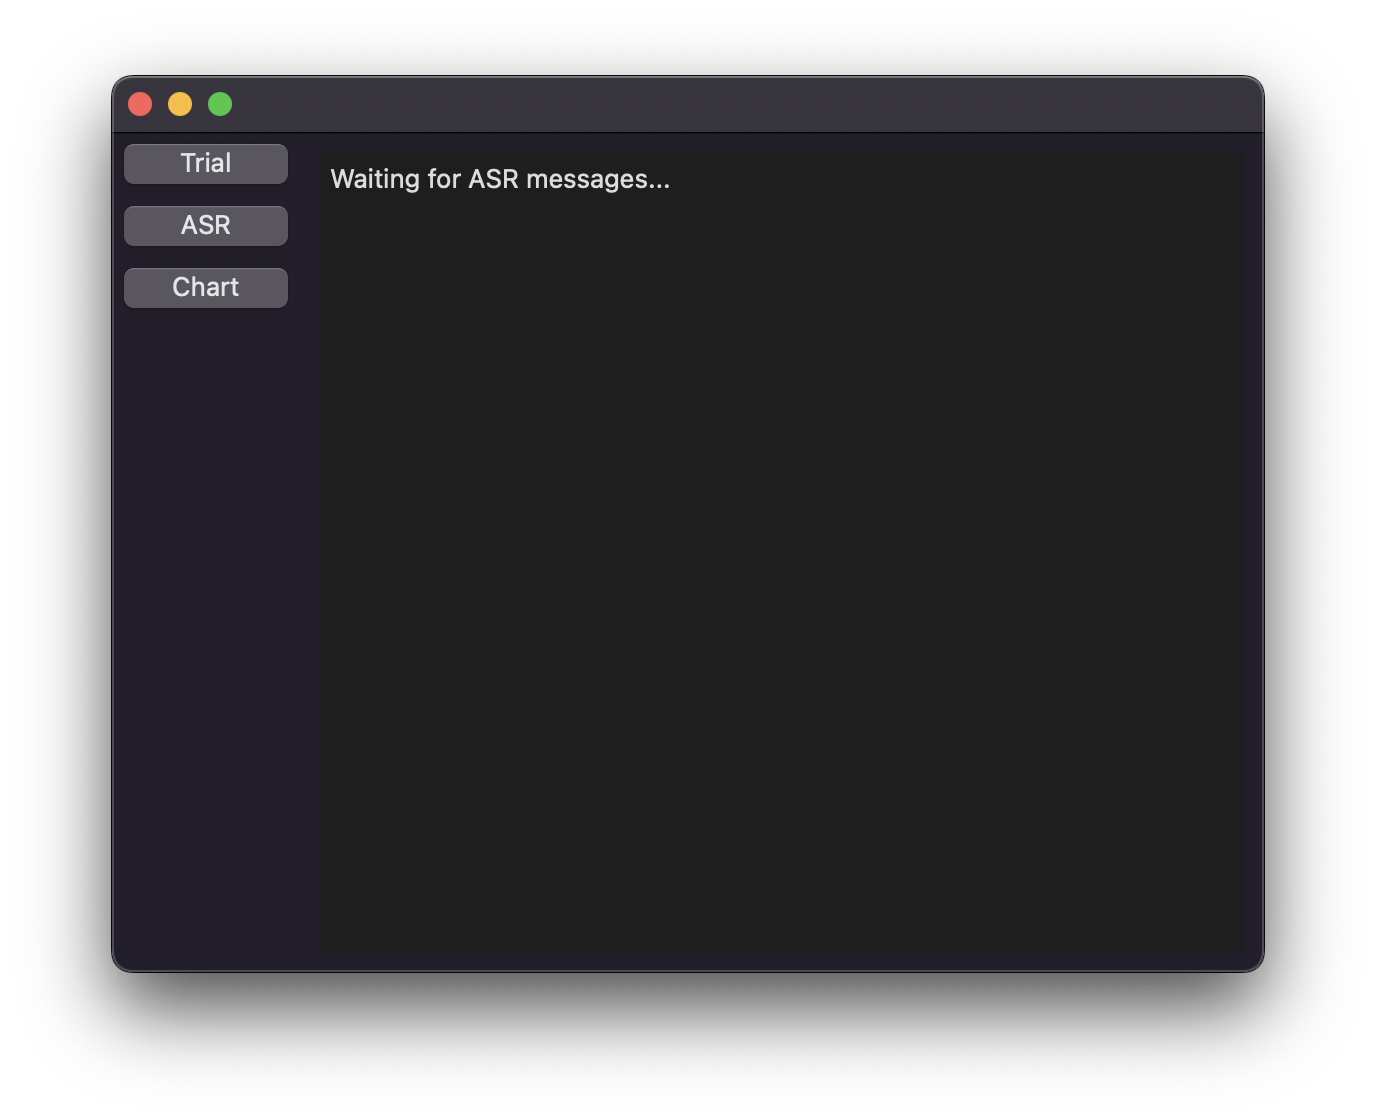
\includegraphics[width=\textwidth]{figures/asr_start}
    \caption{ASR visualization prior to trial start}
    \label{fig:asr_start}
\end{figure}

As the trial progresses, and ASR messages come in, they will fill the panel one
line at a time. In addition to the utterance text itself, each line will also
contain a timestamp of when the utterance was generated, and a participant id
colored to match the associated color of the participant. See
\autoref{fig:asr_viz} for an example.

This color can be red, blue, or green, and the mapping between color and
participant comes from the `trial start' message.

\subsection{Dynamically updating charts}

\paragraph{Chart configuration}

The data being charted can be configured by modifying the ``ChartWidget''
section in \texttt{config/config.json}.

\begin{minted}{JSON}
"ChartWidget":{
    "topics":["score"],
    "x_axis_field": "Time",
    "x_axis_label": "Time",
    "y_axis_field": "Score",
    "y_axis_label": "Score",
    "panel_name": "CHART_PANEL"
 }
\end{minted}

The dashboard will listen for incoming messages on any topics listed in the
``topics'' field. When processing messages, it will then check for the fields
defined by ``x\_axis\_field'' and ``y\_axis\_field”, create an x/y point, and
add that point to the chart. ``x\_axis\_label'' and ``y\_axis\_label'' are used to
add a label to the x-axis and y-axis of the chart. Finally, ``panel\_name'' is
used internally by the dashboard, and should not be modified.  

Below is an example of a `chart' message.

\begin{minted}{JSON}
{
    "data":{
        "Time": 0.2,
        "Score": 10
    }
}
\end{minted}

Notes:

\begin{enumerate}

    \item The ``Time” and ``Score” fields are not at the root level of the JSON
        message, but a part of the ``data” field. This is to keep the
        formatting consistent with for other message types used by the
        dashboard.

    \item Each message should contain exactly one x/y pair. Other fields can be
        included, but will be ignored.

    \item Data points should be either an integer or float value.

\end{enumerate}

To visualize data being charted, navigate to the ``Chart'' tab in the menu
sidebar. At the start of the trial, the right-side panel will display an empty
graph (see \autoref{fig:chart_start}). If a label for the x-axis or y-axis was
defined in the configuration, those labels will be displayed on the axes.  By
default, the graph will be centered around point (0,0). 

\begin{figure}
    \centering
    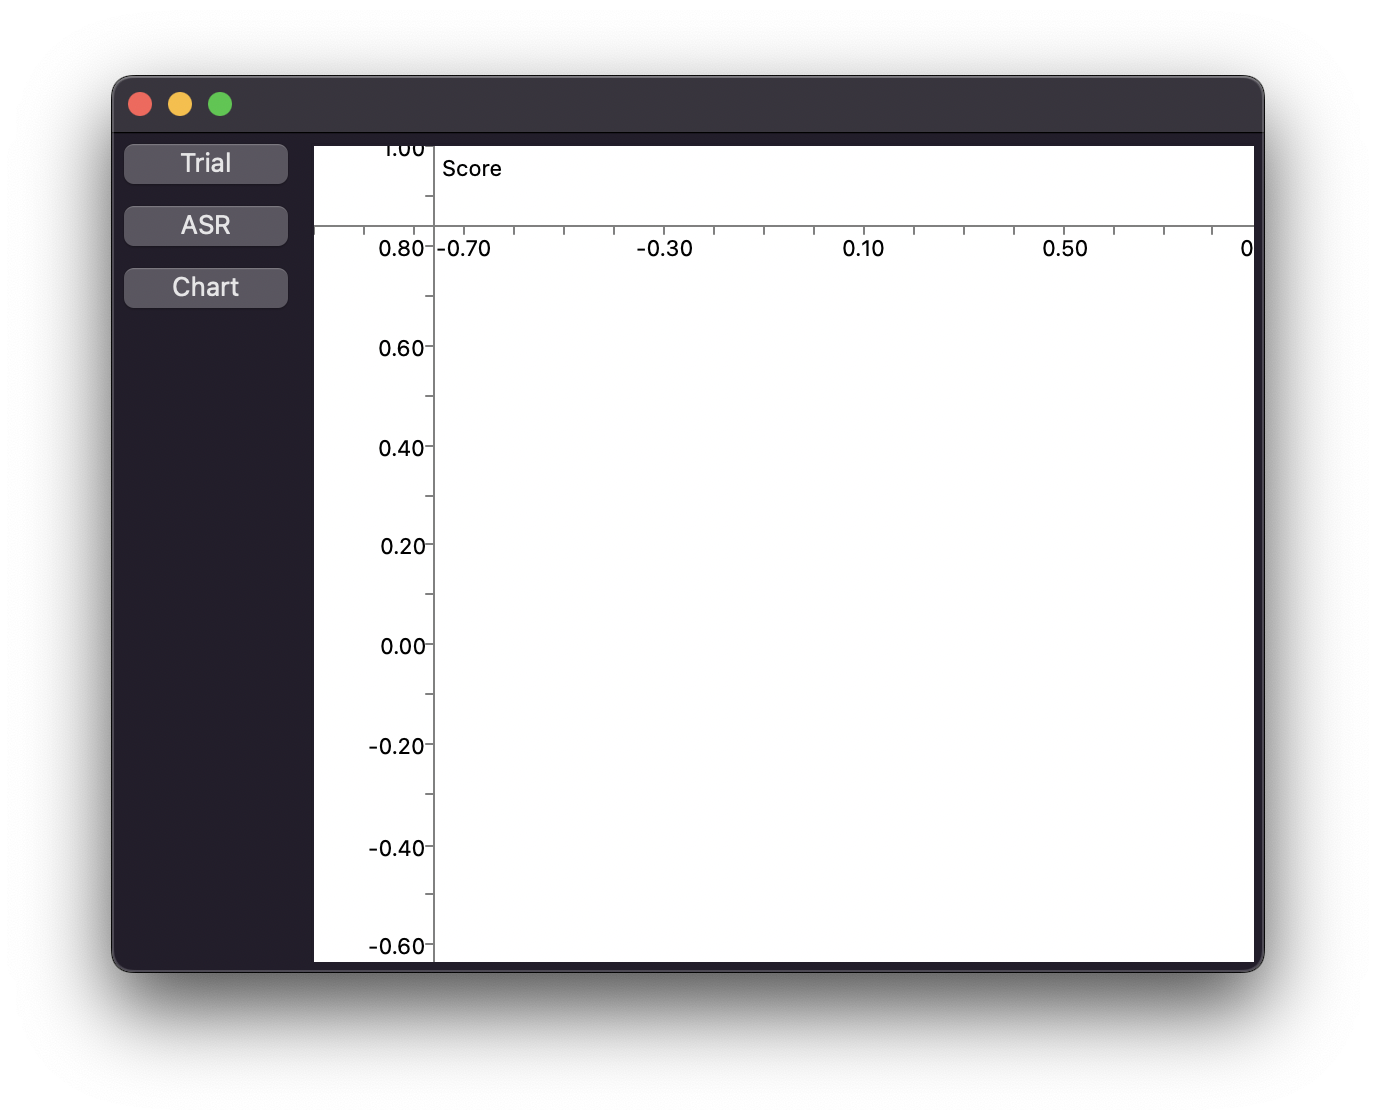
\includegraphics[width=\textwidth]{figures/chart_start}
    \caption{Chart visualization before trial start}
    \label{fig:chart_start}
\end{figure}

When adding a data point, if the data point is outside the visible range, the
chart will automatically fit the data and adjust the x-axis and y-axis so that
the new data point can be seen.

\begin{figure}
    \centering
    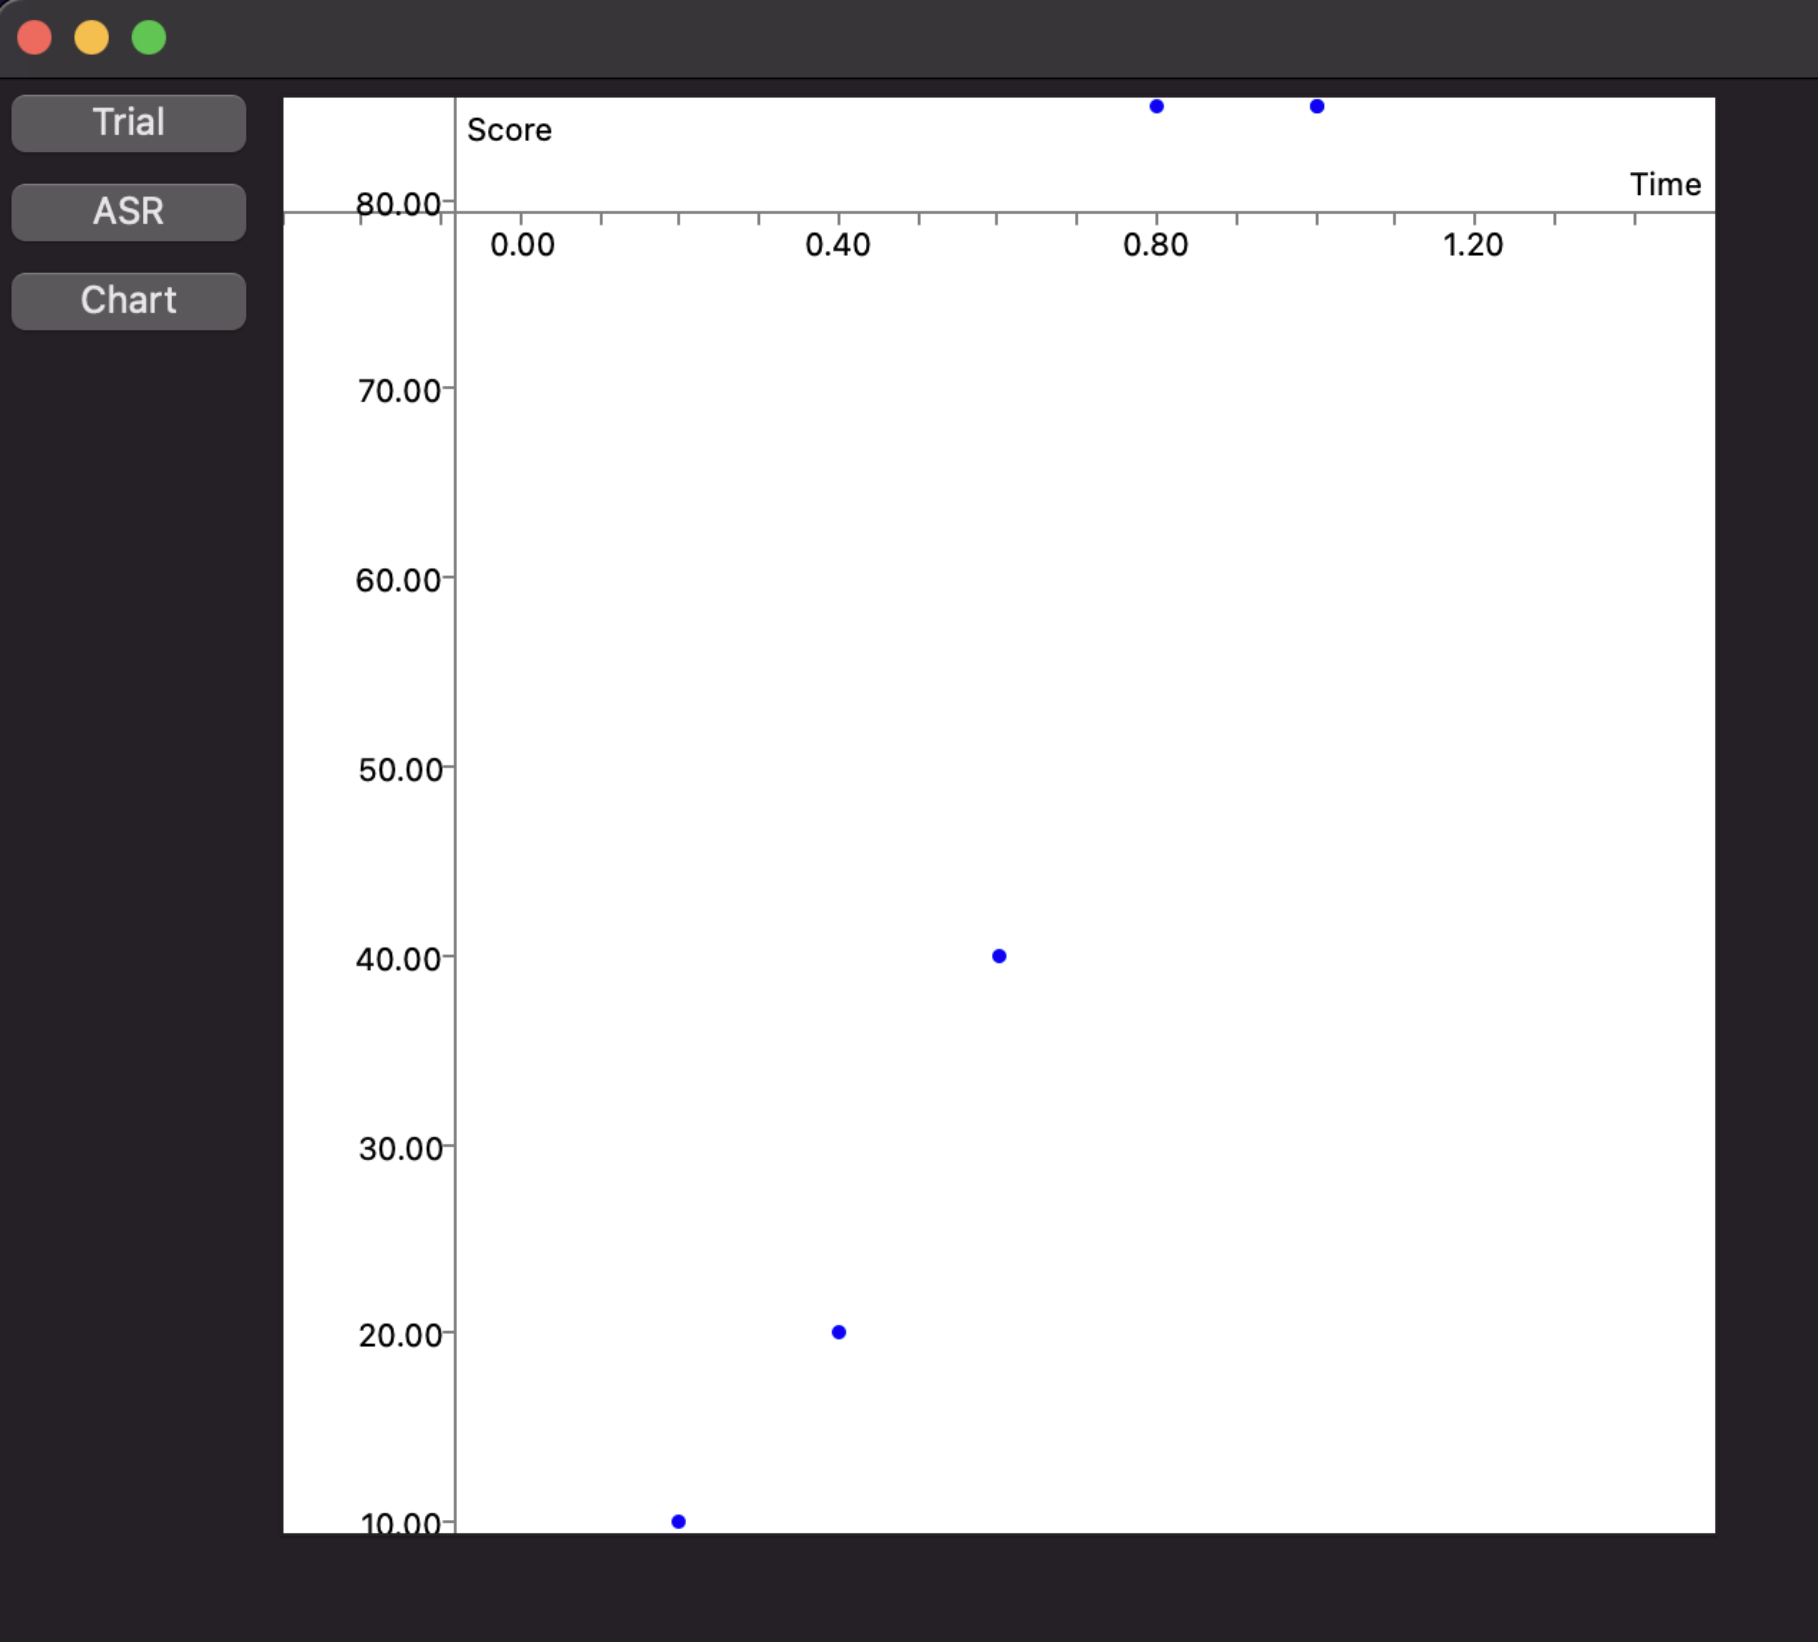
\includegraphics[width=0.8\textwidth]{figures/chart_realtime}
    \caption{Chart visualization during ongoing trial}
    \label{fig:chart_ongoing}
\end{figure}
